\section{Interaction Patterns Between Ase1 and Dynamic Microtubules}
\label{sec:Ase1}

\subsection{The effect of Ase1 crosslinking on the lifetimes of different microtubule overlaps}
\begin{figure}[h]
    \centering
    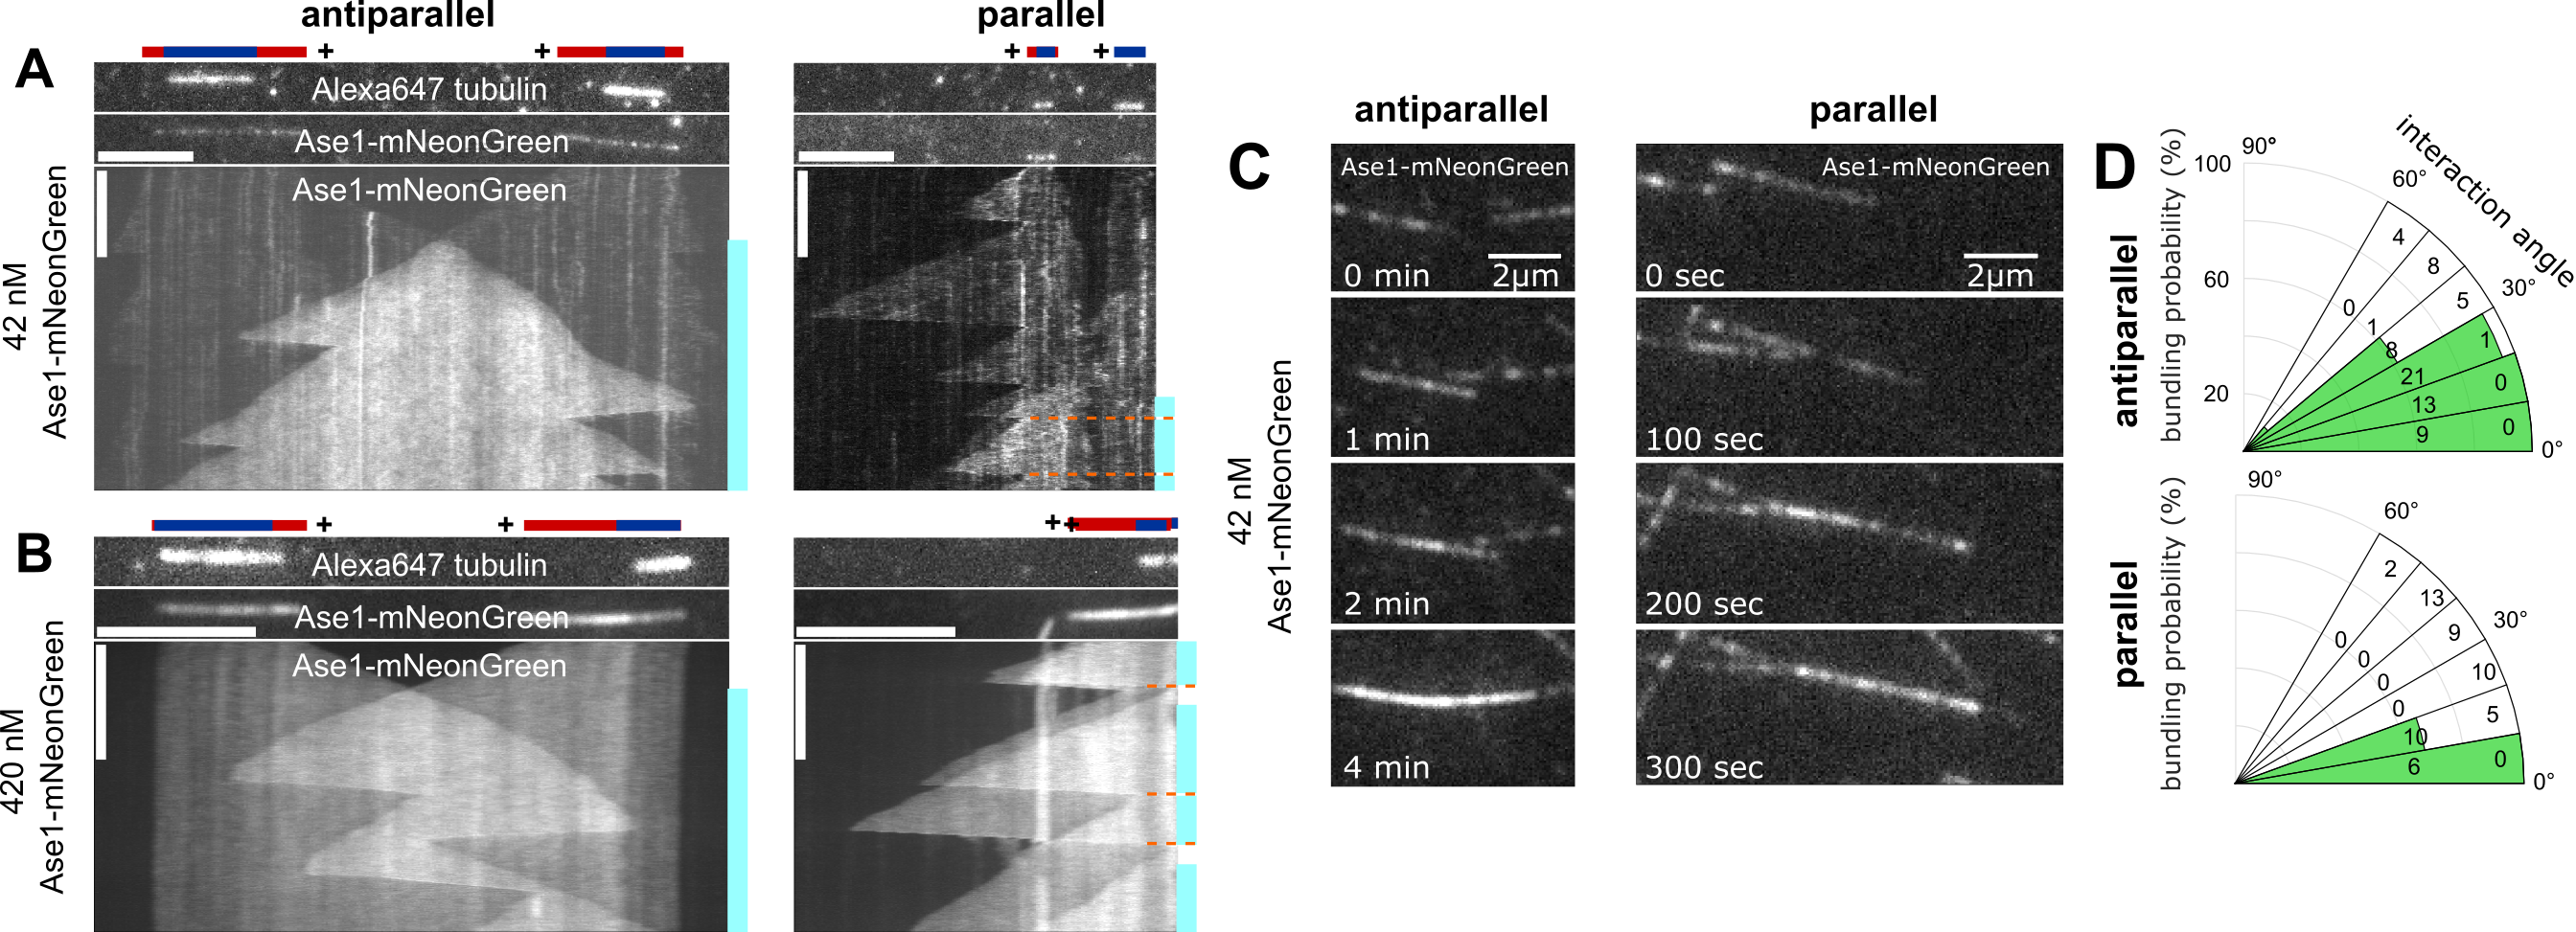
\includegraphics[width=1\linewidth]{Figures/ase1_1a.png}
    \caption[With dynamic microtubule extensions and Ase1, we observed microtubule bundling as previously reported.]{
    (A) Kymographs of an antiparallel (left panel) and a parallel microtubule overlap forming due to the microtubules polymerizing such to enable bundling by Ase1, which is present in solution (42nM). The scale bars are 5 micron and 10 minutes. In sketches, dynamic extensions with GDP lattices are red, and stabilized GMPCPP seeds are blue. The teal bars next to kymographs indicate the presence of regions of overlap (we only counted regions where the two partaking microtubule regions are constituted by GDP-tubulin, i.e., a seed stabilized by GMPCPP did not count). The orange lines indicate a termination of the overlapping period, as evaluated for \autoref{ase1b}A. (B) Same representation as A showing events from experiments performed at 420nM Ase1. (C) Snapshots of different events than shown in A and B, illustrating microtubule bundling (at 42nM). (D) Bundling probability for situations when microtubule plus ends encountered other microtubules, in either parallel or antiparallel orientation, versus the initial angle of interaction (results pooled for all Ase1-mNeonGreen concentrations). The outer numbers denote the numbers of recorded crossings at the respective angle, while the inner numbers denote the numbers of bundling events (the sum of both numbers is the total number of observed events).
        }\label{ase1a}
\end{figure}
To investigate the interactions between diffusible microtubule (microtubule) crosslinkers and depolymerizing microtubule ends, we employed total internal reflection fluorescence (TIRF) time-lapse imaging of immobilized, GMPCPP-stabilized microtubule seeds in the presence of 30 µM free tubulin and varying concentrations of Ase1. At concentrations of 42 nM and 420 nM Ase1, we observed dynamic, Ase1-decorated microtubule extensions polymerizing from the microtubule seeds \pref{ase1a}{A,B}. When two microtubule plus ends, emanating from different seeds and polymerizing towards each other, encountered each other, the microtubules either bundled or crossed, depending on the angle of incidence. Typically, at high angles, the microtubules crossed and only interacted at the crossing point, while at small angles, either parallel or antiparallel associations could be formed \pref{ase1a}{C}. As previously reported \parencite{Janson2007}, antiparallel bundles formed even at large initial angles of incidence (up to 40°), while parallel bundles only formed at initial angles below 20° \pref{ase1a}{D}.\par
\begin{wrapfigure}{l}{0.4\textwidth}
    \centering
    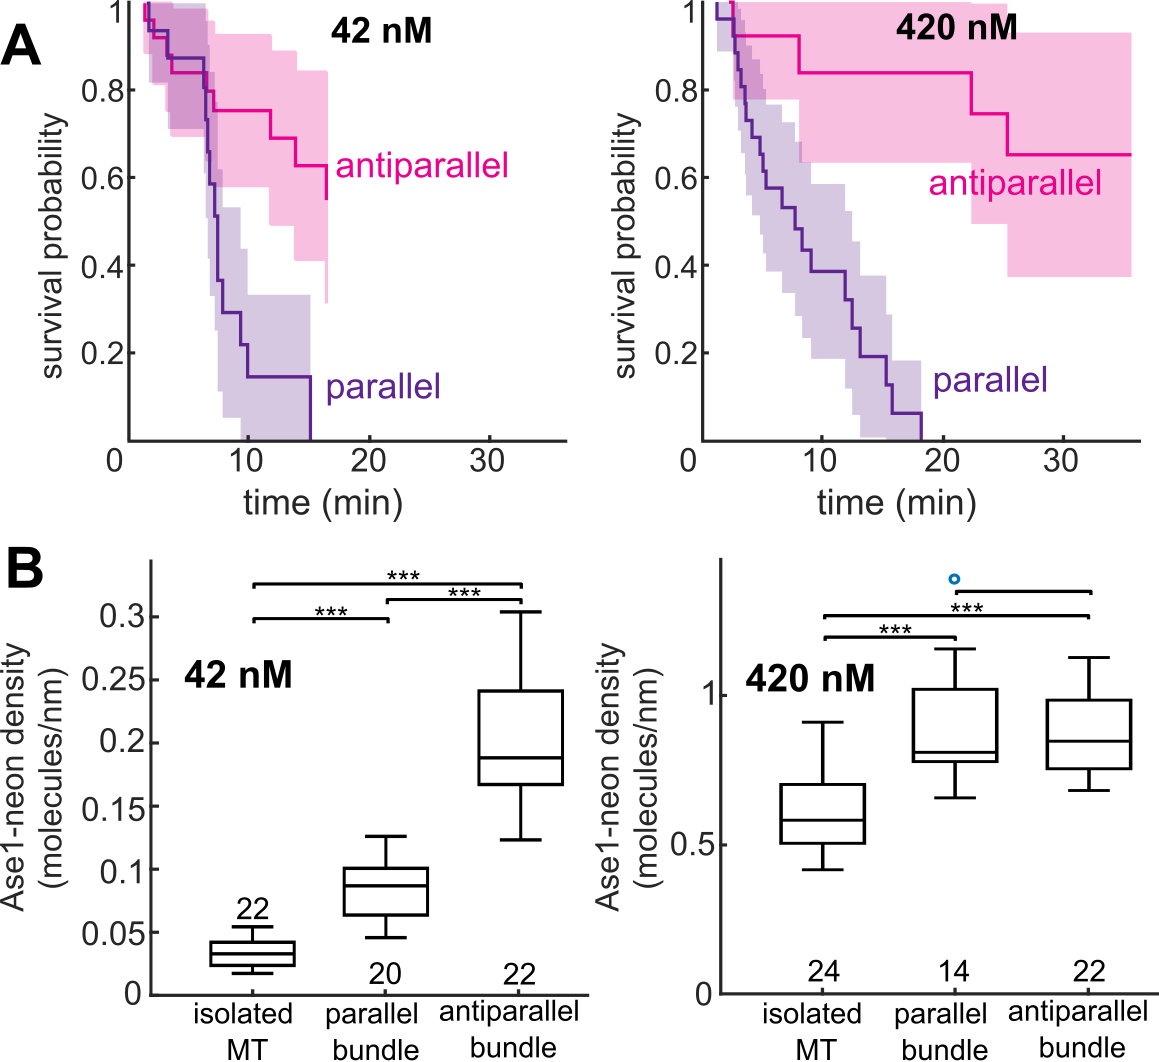
\includegraphics[width=1\linewidth]{Figures/ase1_1b.png}
    \caption[Ase1 selectively stabilizes antiparallel overlaps.]{
    (A) Survival probability of antiparallel and parallel overlaps, showing the probability that an overlap formed by two dynamic MT extensions persists at a given time after its formation (Methods). Semitransparent regions indicate 95\% lower and upper confidence bounds. (B) Quantification of the density of Ase1-mNeonGreen on isolated MTs and (anti)parallel bundles (Methods). The numbers below the boxes denote the number of analyzed microtubule bundles. Panels show data for MT plus ends (minus ends generally were not analyzed). 
        }\label{ase1b}
\end{wrapfigure}
Quantitative analysis revealed increased lifetimes of antiparallel overlaps compared to parallel ones\pref{ase1b}{A} Notably, at 42 nM Ase1 in solution, the Ase1 density on antiparallel overlaps was an order of magnitude higher than on parallel ones\pref{ase1b}{B} consistent with the previously reported differential affinities \parencite{Janson2007}. At 420 nM Ase1, we observed the density of Ase1 to be similar on antiparallel and parallel bundles, roughly twice the density found on isolated microtubules\pref{ase1b}{B} This possibly indicated that, at this high concentration, a similar number of Ase1 molecules was present within parallel and antiparallel overlaps. Note, however, that this value represents the total density of Ase1 at the bundle, which might differ from the density of Ase1 molecules directly engaged in MT crosslinking by being bound simultaneously to both microtubules. Despite similar decoration levels by Ase1, antiparallel overlaps were still significantly more stable than parallel ones\pref{ase1b}{A} Given the low polymerization velocity of minus ends, we very rarely observed antiparallel overlaps formed by two minus ends encountering each other, and we thus could not meaningfully quantify the associated lifetime. Generally, we chose to not analyze minus ends given that they are not dynamic \textit{in vivo} \parencite{dammer}.\par

To test whether the relative stability of antiparallel overlaps was caused by Ase1 crosslinking or the bundling itself (as was requested by a reviewer), we also conducted experiments at 10nM Ase1. At this concentration, we observed significantly less Ase1 within antiparallel bundles \pref{ase1c}{A}, and indeed, antiparallel bundles were no more stable than parallel bundles \pref{ase1c}{B}. Also, at 10nM Ase1 we observed antiparallel microtubules to no longer bundle as readily as at higher Ase1 concentrations \pref{ase1c}{C}. While we could detect an Ase1 signal at antiparallel overlaps, we did observe events where Ase1 crosslinking apparently was not strong enough to keep a MT plus end bundled to the MT along which it was growing in an antiparallel orientation \pref{ase1c}{D,E left panel}. Finally, to test whether microtubule bundling in our assays was partially a result of molecular crowding (and not Ase1), we performed an assay at 0nM Ase1. In absence of Ase1, microtubules never bundled, even when very close to each other over extended periods of time, indicating that molecular crowding did not play a role in the microtubule bundling we observed \pref{ase1c}{F}. \par

The relative stability of antiparallel overlaps at high Ase1 concentrations may at least partly owe to the fact that antiparallel overlaps grow with twice the speed of parallel overlaps (since both microtubules polymerize in opposite directions, however it should be noted that once a minus end has been surpassed the antiparallel overlaps does no longer grow as quickly on the side in question); hence, there is more opportunities for rescues to occur during depolymerization. However, our kymographs suggested that antiparallel overlaps may be additionally stabilized by an increase in rescue frequency \pref{ase1a}{A,B}, and we set out to quantify this issue next.

\begin{figure}[h]
    \centering
    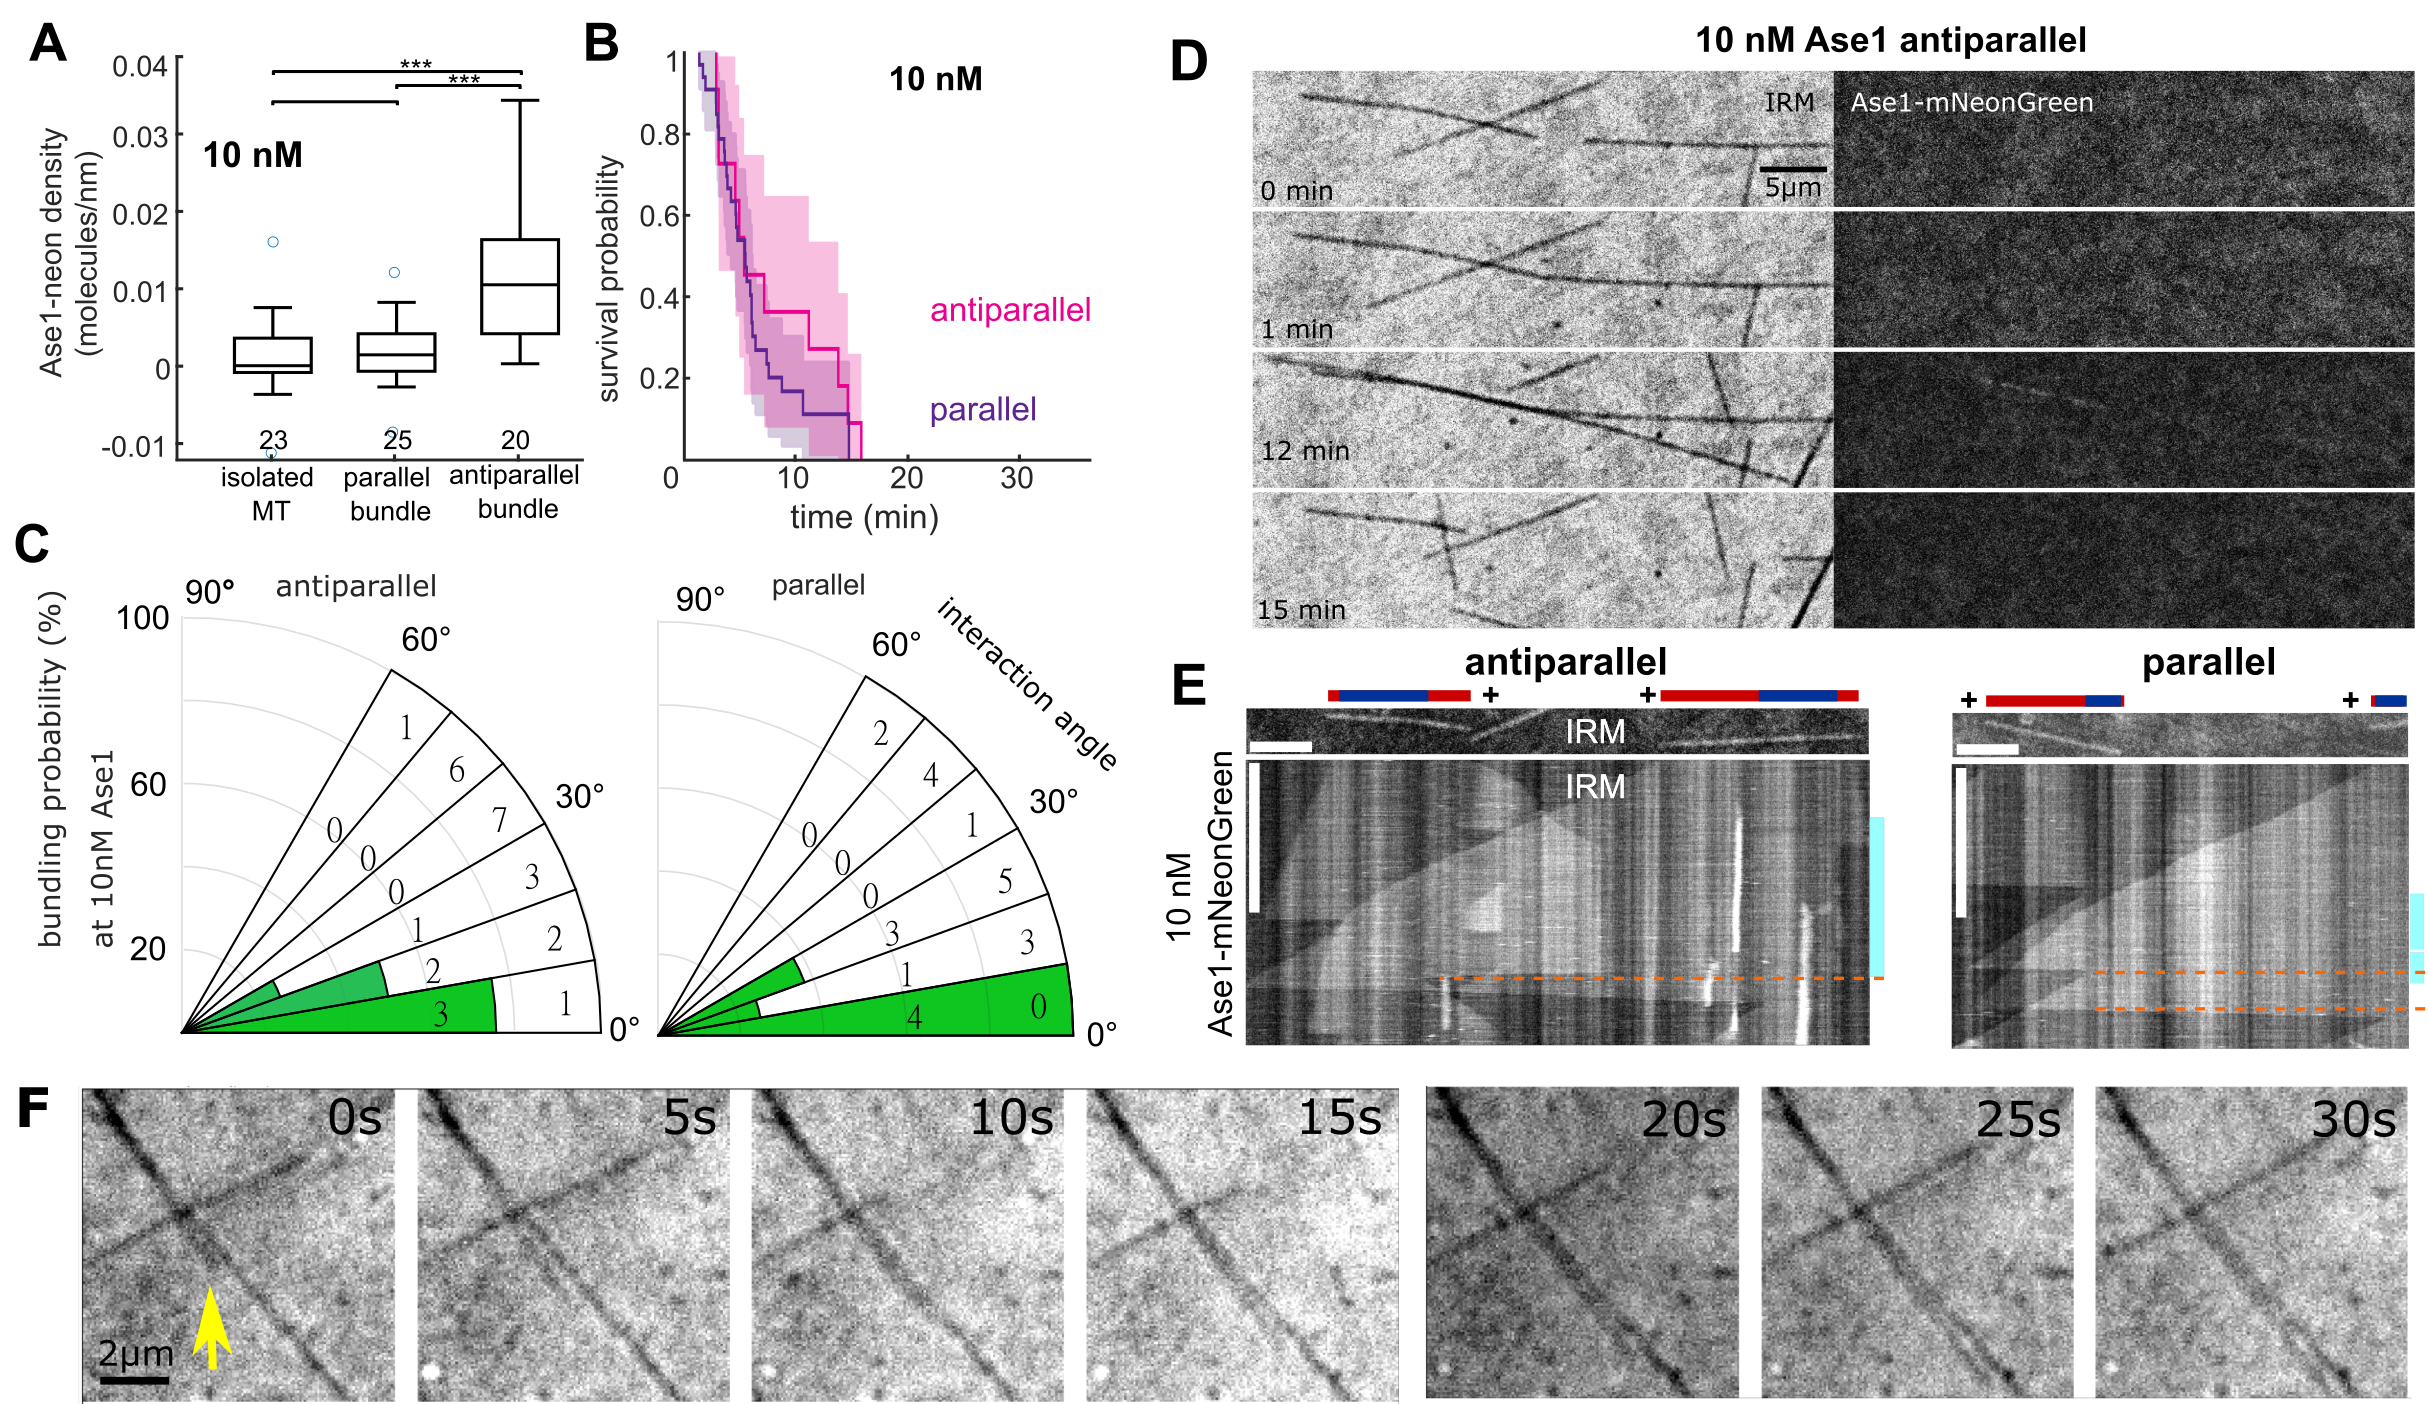
\includegraphics[width=1\linewidth]{Figures/ase1_1c.png}
    \caption[Antiparallel overlaps are not significantly stabilized at low Ase1 concentrations.]{
        (A,B) Quantifications of Ase1 densities and lifetimes for the 10nM Ase1 condition analogous to panels in \autoref{ase1b}. (C) Quantifications of bundling probabilities for the 10nM Ase1 condition analogous to \autoref{ase1a}D. (D) Snapshots of an antiparallel overlap at 10nM Ase1. (E) Kymographs for the 10nM Ase1 condition, representation analogous to \autoref{ase1a}A. The left panel shows the same event as D. (F) A microtubule polymerizing close to another, parallel microtubule at 0nM Ase1 (imaged with IRM). The tip of microtubule in question is indicated by a yellow arrow. As can be seen, no bundling is occurring despite the fact that the microtubules are very close to each other.
        }\label{ase1c}
\end{figure}